%%
%% This is file `sample-sigconf.tex',
%% generated with the docstrip utility.
%%
%% The original source files were:
%%
%% samples.dtx  (with options: `sigconf')
%% 
%% IMPORTANT NOTICE:
%% 
%% For the copyright see the source file.
%% 
%% Any modified versions of this file must be renamed
%% with new filenames distinct from sample-sigconf.tex.
%% 
%% For distribution of the original source see the terms
%% for copying and modification in the file samples.dtx.
%% 
%% This generated file may be distributed as long as the
%% original source files, as listed above, are part of the
%% same distribution. (The sources need not necessarily be
%% in the same archive or directory.)
%%
%%
%% Commands for TeXCount
%TC:macro \cite [option:text,text]
%TC:macro \citep [option:text,text]
%TC:macro \citet [option:text,text]
%TC:envir table 0 1
%TC:envir table* 0 1
%TC:envir tabular [ignore] word
%TC:envir displaymath 0 word
%TC:envir math 0 word
%TC:envir comment 0 0
%%
%%
%% The first command in your LaTeX source must be the \documentclass command.
\documentclass[sigconf]{acmart}

%%
%% \BibTeX command to typeset BibTeX logo in the docs
\AtBeginDocument{%
  \providecommand\BibTeX{{%
    Bib\TeX}}}

%% Rights management information.  This information is sent to you
%% when you complete the rights form.  These commands have SAMPLE
%% values in them; it is your responsibility as an author to replace
%% the commands and values with those provided to you when you
%% complete the rights form.
\setcopyright{acmcopyright}
\copyrightyear{2022}
\acmYear{2022}
\acmDOI{XXXXXXX.XXXXXXX}

%% These commands are for a PROCEEDINGS abstract or paper.
\acmConference[Conference acronym 'XX]{Make sure to enter the correct
  conference title from your rights confirmation emai}{June 03--05,
  2018}{Woodstock, NY}
\acmPrice{15.00}
\acmISBN{978-1-4503-XXXX-X/18/06}

%%
%% Submission ID.
%% Use this when submitting an article to a sponsored event. You'll
%% receive a unique submission ID from the organizers
%% of the event, and this ID should be used as the parameter to this command.
%%\acmSubmissionID{123-A56-BU3}

%%
%% For managing citations, it is recommended to use bibliography
%% files in BibTeX format.
%%
%% You can then either use BibTeX with the ACM-Reference-Format style,
%% or BibLaTeX with the acmnumeric or acmauthoryear sytles, that include
%% support for advanced citation of software artefact from the
%% biblatex-software package, also separately available on CTAN.
%%
%% Look at the sample-*-biblatex.tex files for templates showcasing
%% the biblatex styles.
%%

%%
%% The majority of ACM publications use numbered citations and
%% references.  The command \citestyle{authoryear} switches to the
%% "author year" style.
%%
%% If you are preparing content for an event
%% sponsored by ACM SIGGRAPH, you must use the "author year" style of
%% citations and references.
%% Uncommenting
%% the next command will enable that style.
\citestyle{acmauthoryear}
\setcitestyle{square}

%%
%% end of the preamble, start of the body of the document source.
\begin{document}

%%
%% The "title" command has an optional parameter,
%% allowing the author to define a "short title" to be used in page headers.
\title{Floagent: Interaction with Mid-Air Image via Hidden Sensors}

%%
%% The "author" command and its associated commands are used to define
%% the authors and their affiliations.
%% Of note is the shared affiliation of the first two authors, and the
%% "authornote" and "authornotemark" commands
%% used to denote shared contribution to the research.
\author{Shohei Ando}
\email{ando@media.lab.uec.ac.jp}
\orcid{1234-5678-9012}
\affiliation{%
  \institution{University of Electro-Communications}
  \streetaddress{P.O. Box 1212}
  \city{Chofu}
  \state{Tokyo}
  \country{Japan}
  \postcode{43017-6221}
}

\author{Naoya Koizumi}
\email{koizumi.naoya@uec.ac.jp}
\orcid{1234-5678-9012}
\affiliation{%
  \institution{University of Electro-Communications}
  \streetaddress{P.O. Box 1212}
  \city{Chofu}
  \state{Tokyo}
  \country{Japan}
  \postcode{43017-6221}
}

%%
%% By default, the full list of authors will be used in the page
%% headers. Often, this list is too long, and will overlap
%% other information printed in the page headers. This command allows
%% the author to define a more concise list
%% of authors' names for this purpose.
\renewcommand{\shortauthors}{Trovato et al.}

%%
%% The abstract is a short summary of the work to be presented in the
%% article.
\begin{abstract}
  This paper proposes Floagent as a human-computer interaction system that displays images in mid-air using infrared light reflected by a hot mirror. 
  Floagent is an interaction system that allows users to focus on mid-air images without being aware of the sensors.
  By combining a hot mirror and a retroreflective transmissive optical element, Floagent conceals the camera from the user without affecting the mid-air image.
  We investigated the touch input interactions accuracy with mid-air images to evaluate the proposed system. 
  The results show that the proposed system can effectively measure user input.
  Floagent enables an interaction design with a hidden sensor in which mid-air images appear to respond spontaneously to a wide variety of interaction events. 
\end{abstract}

%%
%% The code below is generated by the tool at http://dl.acm.org/ccs.cfm.
%% Please copy and paste the code instead of the example below.
%%
\begin{CCSXML}
<ccs2012>
 <concept>
  <concept_id>10010520.10010553.10010562</concept_id>
  <concept_desc>Computer systems organization~Embedded systems</concept_desc>
  <concept_significance>500</concept_significance>
 </concept>
 <concept>
  <concept_id>10010520.10010575.10010755</concept_id>
  <concept_desc>Computer systems organization~Redundancy</concept_desc>
  <concept_significance>300</concept_significance>
 </concept>
 <concept>
  <concept_id>10010520.10010553.10010554</concept_id>
  <concept_desc>Computer systems organization~Robotics</concept_desc>
  <concept_significance>100</concept_significance>
 </concept>
 <concept>
  <concept_id>10003033.10003083.10003095</concept_id>
  <concept_desc>Networks~Network reliability</concept_desc>
  <concept_significance>100</concept_significance>
 </concept>
</ccs2012>
\end{CCSXML}

\ccsdesc[500]{Hardware~Display and imagers}
\ccsdesc[100]{Human-centerd computing~Display and imagers}

%\ccsdesc[500]{Computer systems organization~Embedded systems}
%\ccsdesc[300]{Computer systems organization~Redundancy}
%\ccsdesc{Computer systems organization~Robotics}
%\ccsdesc[100]{Networks~Network reliability}

%%
%% Keywords. The author(s) should pick words that accurately describe
%% the work being presented. Separate the keywords with commas.
\keywords{mid-air interaction, augmented reality, mid-air image}
%% A "teaser" image appears between the author and affiliation
%% information and the body of the document, and typically spans the
%% page.
\begin{teaserfigure}
  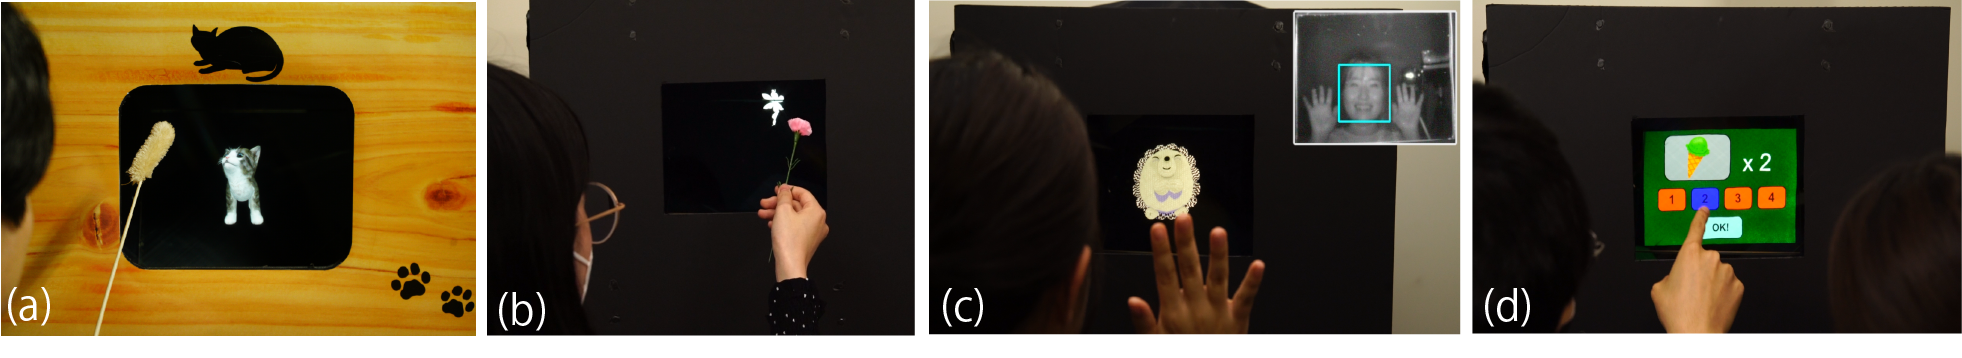
\includegraphics[width=\textwidth]{images/teaser.png}
  \vspace{-2\baselineskip}
  \caption{(a)(b) Interaction with a character displayed as a mid-air image with an object without any sensors (c) Peek-a-boo game with a character displayed in mid-air played via a hidden IR camera (d) Mid-air touch interaction by a user's finger}
  \vspace{0.5\baselineskip}
  \Description{In (a), the user interacts with an image of a cat displayed in mid-air using a cat toy. The cat followed the toy with eyes.
  In (b), the user interacts with a floating image of a fairy using a flower. The fairy displayed in mid-air followed the flower.
  In (c), a user shows their face to an image of a character displayed in mid-air, and the character smiles in response.
  This is called a ``peek-a-boo'' interaction. A photograph of the user's face. recorded by the interior IR camera, is shown.
  In (d), two users touch an interface displayed as a mid-air image.
  The user is shown selecting several items on a meal menu.}
  \label{teaser}
\end{teaserfigure}

%%
%% This command processes the author and affiliation and title
%% information and builds the first part of the formatted document.
\maketitle

\section{Introduction \label{intro}}

In this study, we aim to realize communication with characters and images displayed in mid-air, as popularized in science fiction and fantasy.
In particular, we aim to provide an interaction mechanism that users perceive as ``magical'' to create a dramatically novel human-computer interaction experience.
Although methods to display computer graphics (CG) images floating in mid-air images have been developed, the equipment comprising these systems, such as sensors, is typically visible to users, which considerably detracts from the special experiences commonly shown in fictional media.
We propose Floagent as a system that allows users to interact with mid-air images as if no sensors were present, which uses a micro-mirror array plate (MMAP) device to display mid-air images in real space.
The MMAP comprises two orthogonal mirror arrays. The light emitted from the source is reflected by the MMAP to form a real image in the air.
The mid-air images thus formed can be observed with the naked eye without wearing a device such as an HMD, and can be observed by multiple people simultaneously.

Because mid-air images are formed at some distance from the hardware, research interest in developing non-contact interface methods to prevent the spread of COVID-19 has increased.
However, because such mid-air images lack any physical substance to touch beyond the light reflected in the air, user touch must be detected using non-contact sensors, such as cameras.
MARIO\cite{MARIO} used a depth camera to measure the position of objects and enabled interaction with mid-air images through objects.
Similarly, Chan \textit{et al.}\cite{Void} used an IR camera to measure the positions of the user's finger and projected a shadow to aid interaction.
Additionally, Hunter\textit{et al.}\cite{Seth} solved the occlusion problem when interacting with mid-air images using sensing fingers.

In such mid-air image interaction systems, the quality of the user experience with mid-air images may decrease if the user discovers the sensors.
Alternatively, the equipment comprising the system should be invisible for the user to enjoy the experience with mid-air images as a magician hides tricks.
Hence, sensors, such as cameras, should be positioned in unrecognizable positions to enable a ``magical'' experience.

The proposed system shields the sensors from users using infrared light reflected by a hot mirror.
A hot mirror is an optical element that transmits visible light and reflects only infrared light.
The combined system, comprising a hot mirror and an MMAP unit, hides the camera in the visible light region and creates an experience that enables interaction with a magical mid-air images.

\section{System design \label{proposed}}

Floagent consists of an IR sensor, a display, an MMAP, a hot mirror, and a light shield, as shown in Fig. \ref{fig:hot-MMAPs}.
The light emitted from the display is reflected by the MMAP, which is tilted at a $45^\circ$ angle and forms mid-air images at a position that is plane-symmetrical to the MMAP.
The light that forms the mid-air images is unaffected by the hot mirror because the visible light is transmitted through the hot mirror.
In contrast, infrared light is reflected by the hot mirror; therefore, the hot mirror behaves as a mirror in the infrared band.
Thus, the IR sensor measures the user from the position of the virtual IR sensor, as shown in Fig. \ref{fig:hot-MMAPs}.
Moreover, the light shield prevents the user from observing the sensors or the display.
We sent images from the IR sensor to a workstation computer that used the information to control the images displayed by the system.

\begin{figure}[bt]
  \begin{center}
    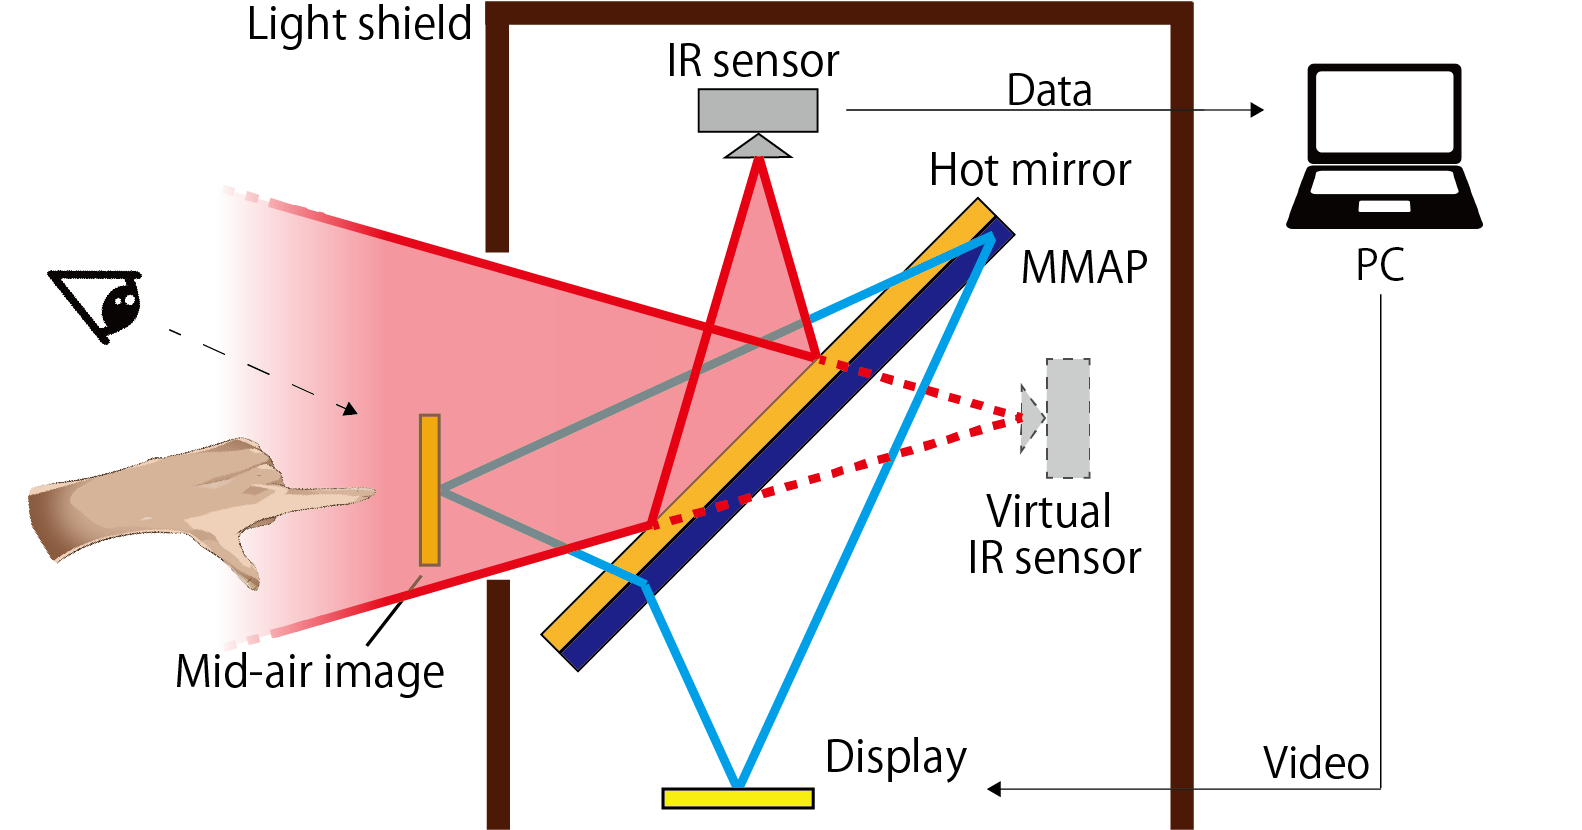
\includegraphics[width=0.8\linewidth]{images/hot-MMAPs_system.png}
    \vspace{-0.8\baselineskip}
    \caption{Optical design and system flow}
    \vspace{-1.5\baselineskip}
    \Description{We show the optical design and system flow of the proposed approach.
    The optical system comprises an IR sensor, a display, an MMAP, a hot mirror, and a light shield.
    The light emitted from the display is reflected by the MMAP, which is tilted at a $45^\circ$  angle and forms mid-air images at a position that is plane-symmetrical to the MMAP.
    Infrared light is reflected by the hot mirror, so the hot mirror functions as a mirror in the infrared band.
    Thus, the IR sensor can measure the user from the virtual IR sensor position.
    Further, because of the light shield, the sensors and the display are hidden from the user.
    Images from the IR sensor are sent to a PC, which uses the information to control the images displayed.}
    \label{fig:hot-MMAPs}
  \end{center}
\end{figure}

\section{Implementation \label{hard}}

The implementation of Floagent is shown in Fig. \ref{fig:opt-sys2}.
An iPad (2048 $\times$ 1536 px) device was used for the display, the MMAP unit was an ASKA3D-488 display (488 mm $\times$ 488 mm, pitch width 0.5 mm) manufactured by ASUKANET, and the hot mirror was a 250 mm $\times$ 250 mm (5 mm thick) unit from Keihin Optical Co.
Because the hot mirror used was smaller than MMAP, its position was adjusted by fitting it to an acrylic plate.
A time-of-flight (ToF) camera from Vzense was used as the IR sensor.
Additionally, the enclosure was covered with blackout curtains and styrene boards to conceal the equipment comprising the system from the user.
In this setup, the infrared light emitted from the ToF camera is reflected by the blackout curtains and interferes with the image captured by the ToF camera.
Therefore, we placed light-absorbing materials inside the blackout curtains to prevent unwanted infrared light reflection.

\begin{figure}[tb]
  \begin{center}
    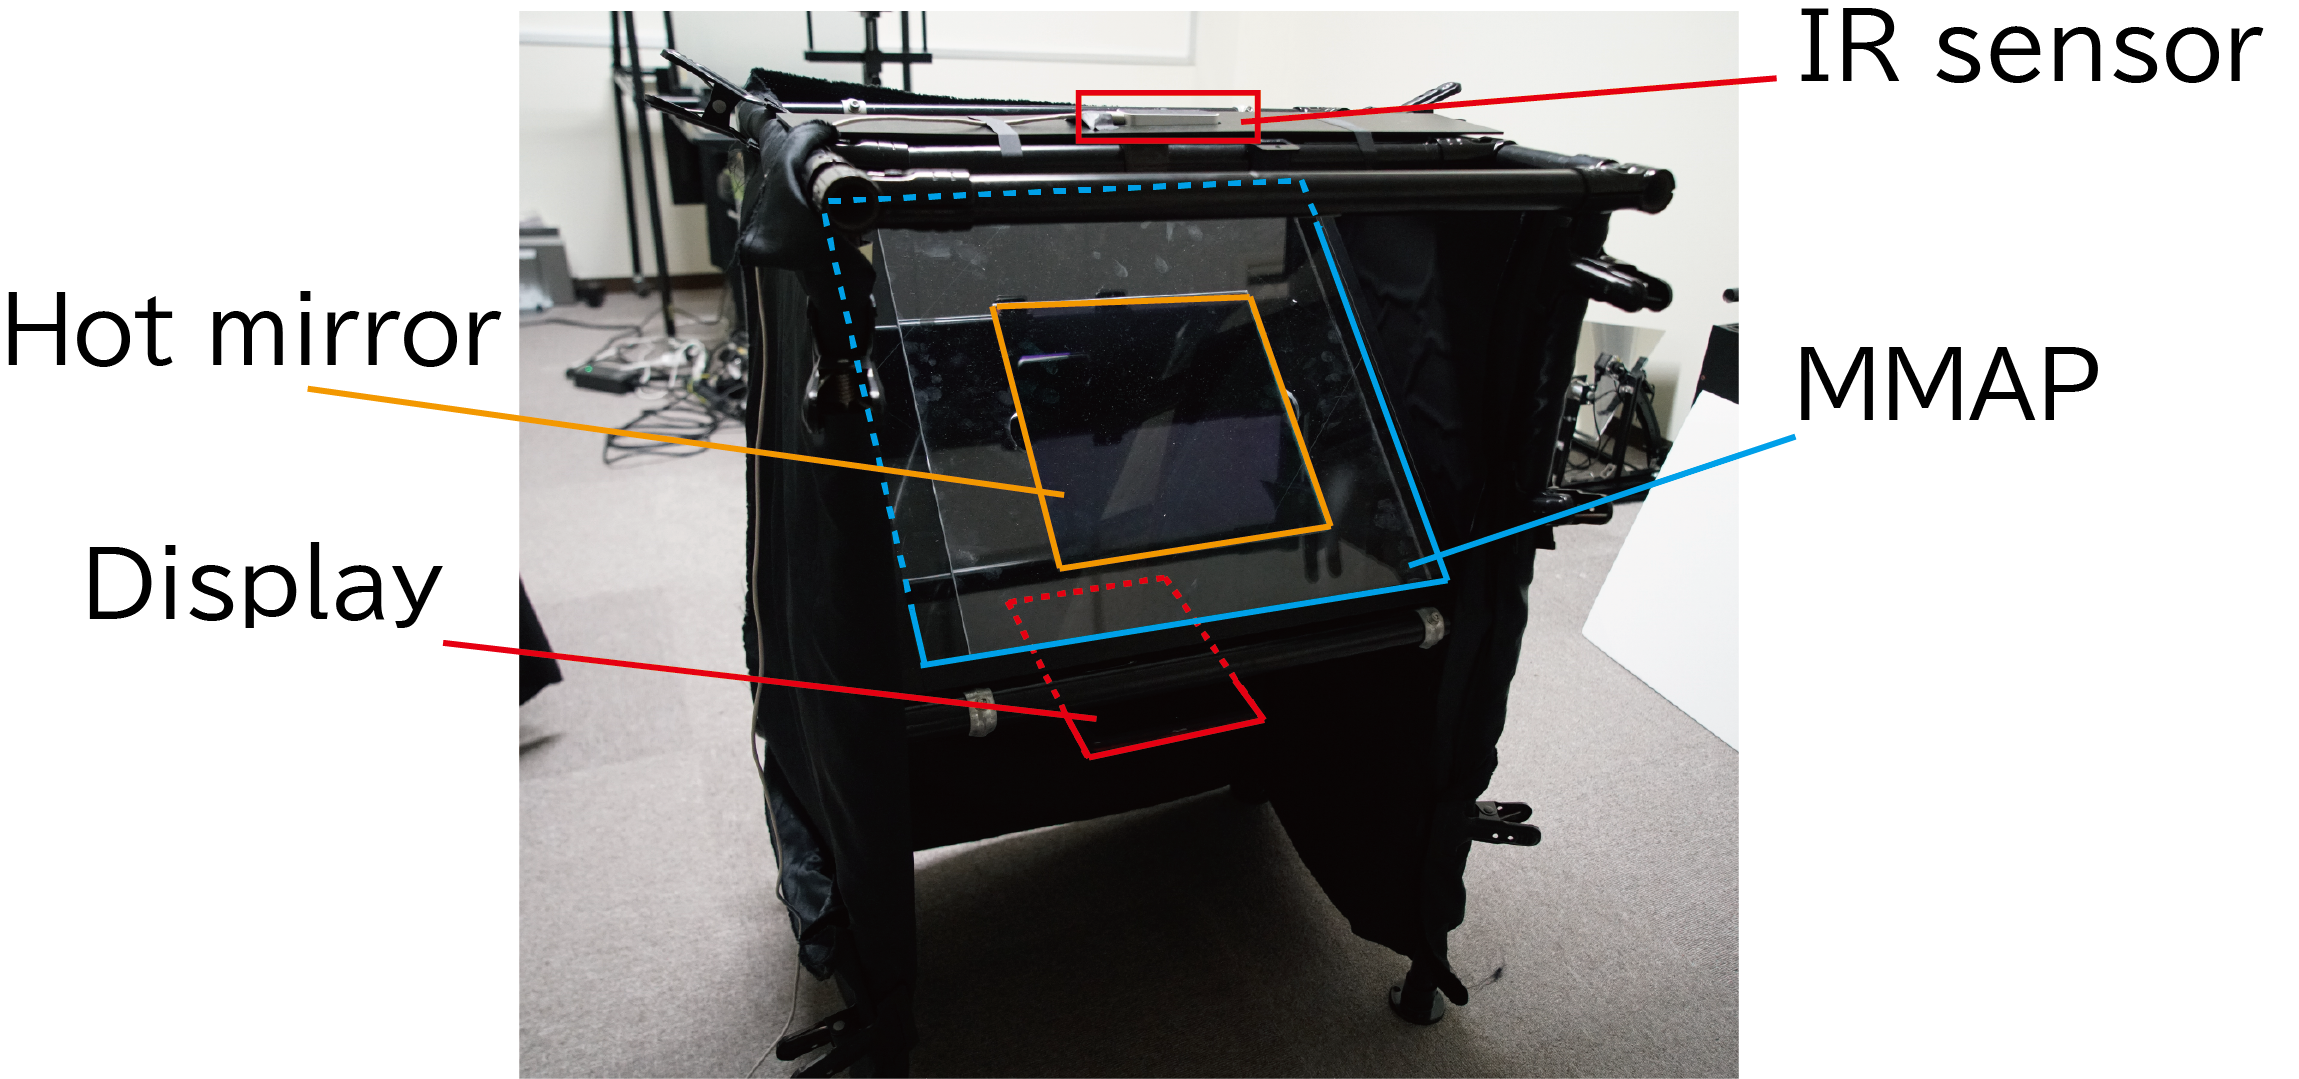
\includegraphics[width=0.8\linewidth]{images/implementation2.png}
    \vspace{-0.9\baselineskip}
    \caption{Implementation}
    \vspace{-1\baselineskip}
    \Description{Front view of the implemented device.
    The hot mirror is located on the MMAP, which is placed at a $45^\circ$ tilt.
    A horizontally positioned display is located below it, and a horizontally positioned IR sensor is located above.
    The equipment is supported by a framework with pipes.}
    \label{fig:opt-sys2}
  \end{center}
\end{figure}

We evaluated the accuracy of finger touch input to the mid-air image display using the implemented device.
The distance error (cm) between the real space and measured coordinates was calculated, and the results are shown in Fig. \ref{fig:result_tof_finger}.
Measurements were recorded at 20 points, and the vertical axis shows the average distance error in cm between the coordinates detected by the touch input system and the true real-space coordinates.
The results show that the maximum median distance error of the coordinates detected by the ToF camera was approximately 2 cm; that is, the error was approximately the width of the fingertip.

\begin{figure}[tb]
  \begin{center}
    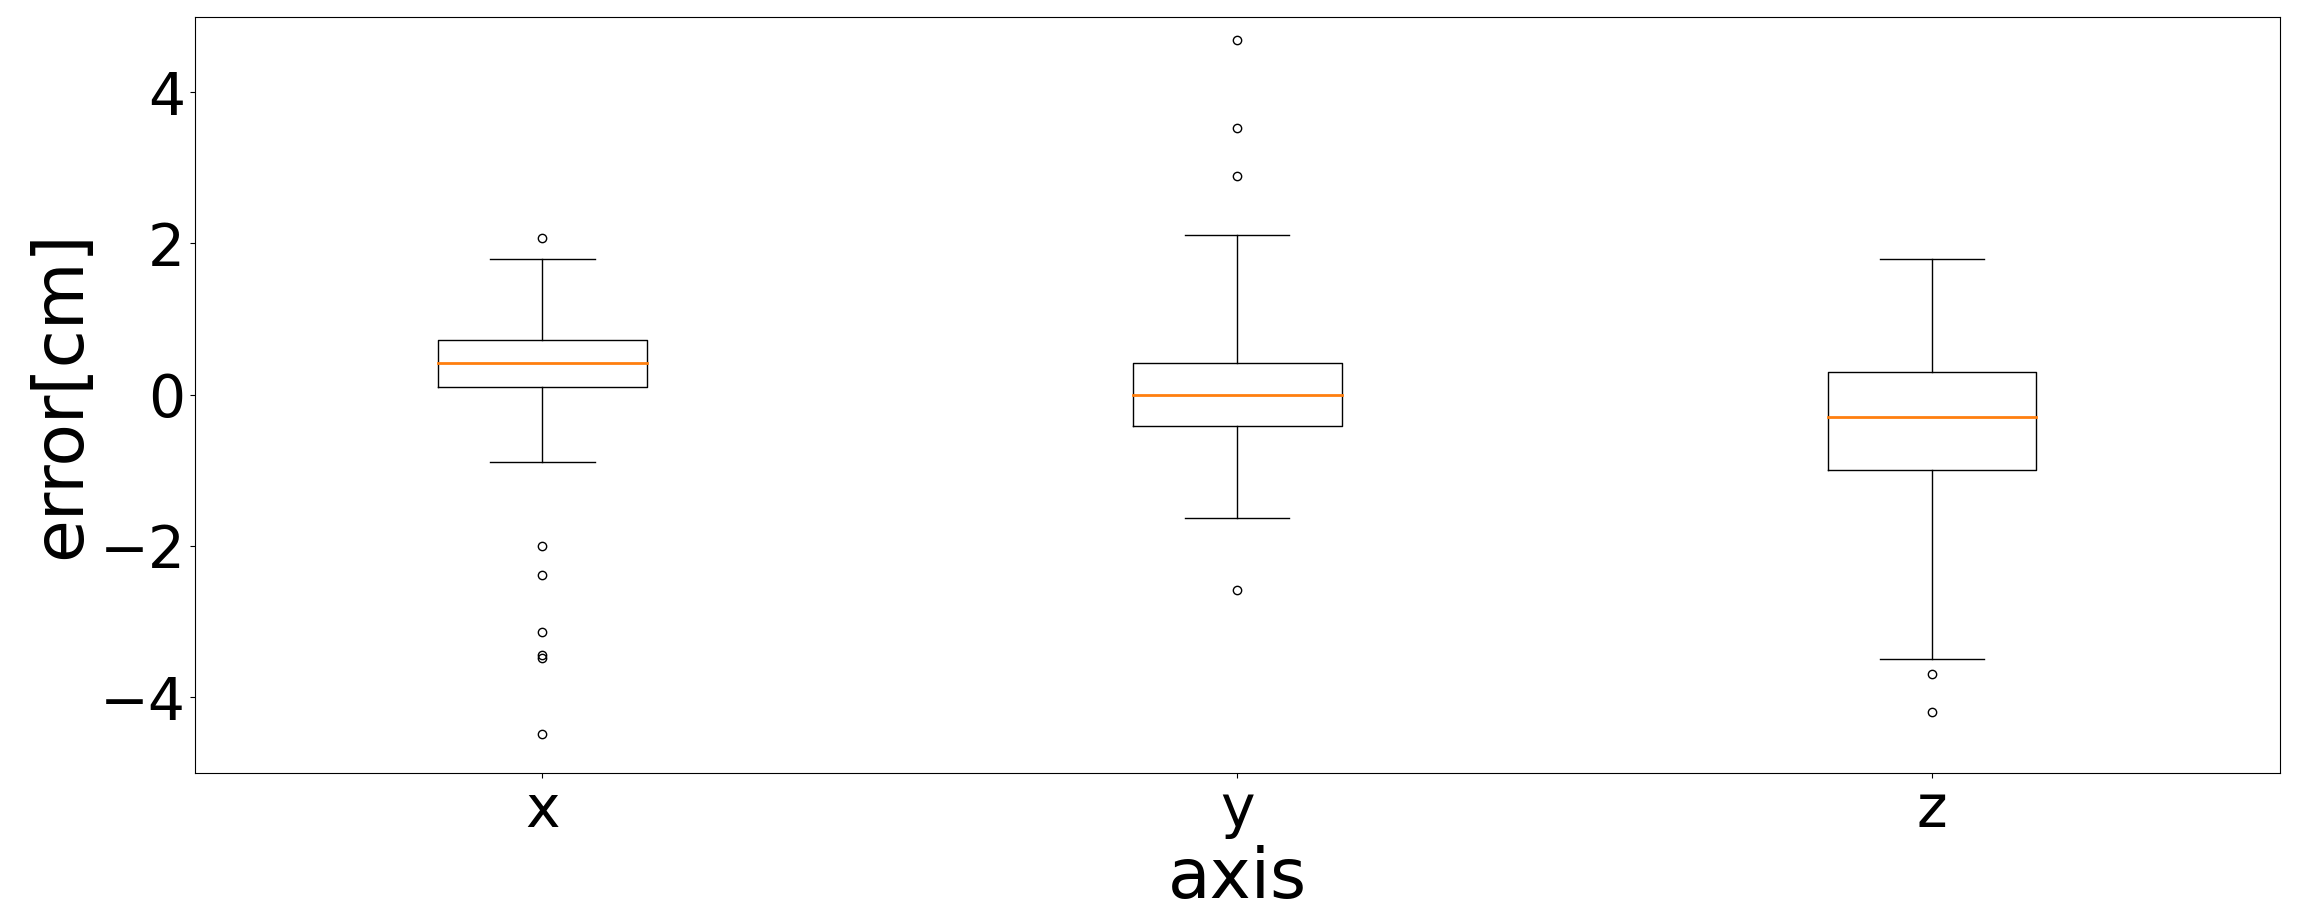
\includegraphics[width=0.8\linewidth]{images/tof_finger_result_ave.png}
    \vspace{-0.9\baselineskip}
    \caption{Results of accuracy evaluation}
    \vspace{-0.9\baselineskip}
    \Description{Box-and-whisker diagram of the results of the accuracy evaluation with finger-touch input to the mid-air image display.
    The horizontal axis shows the x-, y-, and z-axes, and the vertical axis shows the average distance error (cm) between the coordinates detected by a touch input and the real-space coordinates.
    The median value of each was approximately 0 cm and with a maximum value of approximately 2 cm each.
    The minimum values were about -1,2 cm on the x- and y-axes and about -3 cm on the z-axis.
    For the length of the box d, values smaller than the first quartile by over d and exceeding the third quartile by over d are shown as outliers.
    }
    \label{fig:result_tof_finger}
  \end{center}
\end{figure}

\section{Experience \label{consideration}}

Floagent enables the interaction with CG characters using an ordinary object with no sensors, face-to-face communication with mid-air CG characters through face detection by an IR camera, and finger input to interact with interface components, such as touch panels, as shown in Fig \ref{teaser}.
As shown in (a) and (b), the ToF camera was used to detect the position of the tool held by the user, and the animation of the CG character changed according to its position.
Because depth estimation was performed with a ToF camera, the tools need not include sensors, and users can use their fingers as well as objects such as pencils or flowers.
As shown in (c), the CG character reacted when the user's face was detected by the IR camera, realizing a so-called ``peek-a-boo'' game.
As shown in (d), the ToF camera detects the position of the user's finger, allowing the user to operate a mid-air touch panel.
In all of these cases, users can perceive magical images floating in the air without being distracted by special equipment comprising the optical system.

\begin{acks}
  This research was supported by a JSPS Grant-in-Aid JP21K19821 and the Canon Foundation.
\end{acks}

\bibliographystyle{ACM-Reference-Format}
\bibliography{refe}

\end{document}
\endinput